\documentclass[12pt,a4paper]{article}

\usepackage[T1,T2A]{fontenc}
\usepackage[utf8]{inputenc}
\usepackage[english,russian]{babel}
\usepackage{microtype}
\usepackage{csquotes}
\usepackage{amsmath}
\usepackage{amsthm}
\usepackage{amssymb}
\usepackage{mathtext}
\usepackage{physics}
\usepackage{newfloat}
\usepackage{caption}
\usepackage{indentfirst}
\usepackage{titlesec,titletoc}
\usepackage{geometry}
\usepackage{hyperref}
\usepackage{mdframed}
\usepackage[inline]{enumitem}
\usepackage{graphicx}
\usepackage{subfig}
\usepackage[titletoc,toc]{appendix}

\DeclareGraphicsExtensions{.pdf,.png,.jpg,.PNG}
\graphicspath{{./img/}}
\captionsetup[figure]{justification=centering}
\renewcommand{\thesubfigure}{\asbuk{subfigure}}
\DeclareCaptionLabelSeparator{dotseparator}{. }
\captionsetup{labelsep=dotseparator}
\geometry{left=1cm,right=1cm,top=2cm,bottom=2cm}
\makeatletter\appto{\appendices}{\def\Hy@chapapp{Appendix}}\makeatother
\renewcommand{\appendixtocname}{Приложения}
\renewcommand{\appendixpagename}{Приложения}

\DeclareMathOperator{\Rot}{\mathbf{rot}}
\DeclareMathOperator{\Grad}{\mathbf{grad}}
\DeclareMathOperator{\Div}{\mathbf{div}}
\DeclareMathOperator{\D}{D}
\newcommand{\V}[1]{\mathbf{#1}}
\newcommand{\Op}[1]{\hat{\V{#1}}}


\titlelabel{\thetitle. }

\hypersetup{
	colorlinks,
	citecolor=black,
	filecolor=black,
	linkcolor=black,
	urlcolor=black
}

\begin{document}

    \makeatletter
\begin{titlepage}

	\newpage

    \noindent\centering{
    	МИНИСТЕРСТВО ОБРАЗОВАНИЯ И НАУКИ РОССИЙСКОЙ ФЕДЕРАЦИИ

    	Федеральное государственное автономное образовательное учреждение высшего образования \enquote{Нижегородский государственный университет им. Н.И. Лобачевского} (ННГУ)
    }

	\vspace*{50pt}

	Физический факультет \\[\baselineskip]

	Кафедра информационных технологий\\
	в физических исследованиях

	\vspace*{100pt}

	{\Large\textbf{Отчет}} \\
	по преддипломной практике \\[\baselineskip]

	{\Large\textbf{Тепловое излучение в сферическом резонаторе}}

	\vspace*{\fill}

	\hfill\begin{minipage}{15em}
    	Выполнил\\
		студент 4 курса 05144 группы\\
		\textbf{Василевский А.В.}
    \end{minipage} \\[\baselineskip]

	\hfill\begin{minipage}{15em}
    	Научный руководитель\\
		доцент кафедры ИТФИ\\
		к. ф.-м. н.\\
		\textbf{Бурланков Д.Е.}
    \end{minipage}

	\vspace*{\fill}

	Нижний Новгород\par

	\centering{2018 г.}

\end{titlepage}
\makeatother


    \tableofcontents

    \newpage

    %
    %
    %
    %%%%%%%%%%%%%%%%%%%%%%%%%%%%%%%%%%%%%%%%%%%%%%%%%%%%%%%%%%%%%%%%%%%%%%%
    %                           SECTION                                   %
    %%%%%%%%%%%%%%%%%%%%%%%%%%%%%%%%%%%%%%%%%%%%%%%%%%%%%%%%%%%%%%%%%%%%%%%
    %
    %
    %

    \section*{Введение}

        Неотъемлемым элементом почти любого сложного оптического и микроволнового прибора является резонатор. Именно прогресс в совершенствовании резонаторов зачастую приводил к достижению качественно новых результатов. Так, появление мазеров и лазеров было бы невозможно без реализации высокодобротных резонаторов СВЧ и оптического диапазонов. Высокодобротные резонаторы активно используются для сужения и стабилизации линии генерации, в качестве фильтров и дискриминаторов, в разнообразных высокочувствительных сенсорах и датчиках, в метрологии и в прецизионных физических экспериментах. \cite{microresonators}

        Так, одним из ключевых направлений развития физики сегодня является квантовая теория измерений и связанный с ней интерес к манипуляциям с отдельными квантовыми объектами. Резонаторы играют существенную роль в этих исследованиях. Именно с помощью миниатюрных высокодобротных резонаторов в оптическом диапазоне были впервые продемонстрированы неклассические состояния электромагнитного поля и были впервые проведены впечатляющие эксперименты по наблюдению эффектов взаимодействия отдельных фотонов и отдельных атомов. Тесно связаны с этим направлением и такие, вызывающие активное внимание и ожидания, приложения, как квантовые компьютеры, квантовая криптография и квантовая телепортация. Одним из основных требований для наблюдения квантовых эффектов является изоляция системы от внешнего классического мира и уменьшение в ней диссипации для замедления распада состояний (декогеренции), что означает для резонаторов повышение добротности. \cite{microresonators}

        Взаимодействие излучения со сферическими телами исследуется уже более 100 лет. В последние десятилетия, в связи с обнаружением сверхузких резонансов рассеяния и возможностью создания на этой основе микрорезонаторов с гигантской добротностью, открывающих новые горизонты оптической микрофотоники, интерес к этому вопросу усилился многократно. \cite{microresonators}

        Повышенный интерес к микрорезонаторам и бурное развитие области сверхдобротных резонаторов ставят перед наукой и другие задачи. Всесторонний анализ различных путей диссипации энергии в микрорезонаторах с целью повышения их добротности и стабильности является задачей, требующей особого внимания. Для микроэлектронных приборов, элементов квантовых компьютеров и т.д. не менее важным является вопрос устранения шумов. Тепловые шумы являются довольно серьезным мешающим фактором. Генерация этих шумов на сферических микроструктурах тоже требует изучения в целях их учета и компенсации.

        На \autoref{fig:spherical_resonator} показан сферический микрорезонатор с МШГ (моды шепчущей галереи). В виде пояса видна спекл-картина рассеяния на поверхностных неоднородностях поля МШГ.
        %
        \begin{figure}[h]
            \centering
            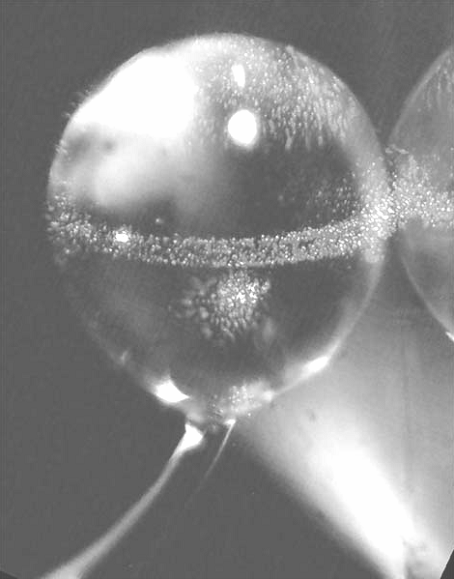
\includegraphics[width=0.5\textwidth]{spherical_resonator}
            \caption[]{Оптический сферический микрорезонатор на ножке рядом с возбуждающей призмой, в которой видно его отражение. Диаметр около $570$ мкм, добротность $> 10^9$. Физический факультет МГУ \cite{microresonators}}
            \label{fig:spherical_resonator}
        \end{figure}

    %
    %
    %
    %%%%%%%%%%%%%%%%%%%%%%%%%%%%%%%%%%%%%%%%%%%%%%%%%%%%%%%%%%%%%%%%%%%%%%%
    %                           SECTION                                   %
    %%%%%%%%%%%%%%%%%%%%%%%%%%%%%%%%%%%%%%%%%%%%%%%%%%%%%%%%%%%%%%%%%%%%%%%
    %
    %
    %

    \section{Постановка задачи}

        Целью данной работы является построение мод электромагнитного поля в сферическом резонаторе и исследование их термодинамики.

        Классические методики решения данной задачи в значительной степени эвристичны, другие приводят к весьма громоздким результатам. К тому же их применение к полям б\'{о}льшей тензорной размерности весьма проблематично. \cite{burlankov_tmf}

        В данной работе приводится новый подход, в основе которого лежат векторы Киллинга пространства, в котором распространяется поле. Данный подход учитывает естественную симметрию объемлющего пространства, тем самым требует более коротких выкладок. К тому же он естественным образом обобщается для описания полей любой тензорной размерности, например гравитационного. \cite{burlankov_tmf}

        Впервые указанная методика была применена для описания полей различной тензорной размерности на трехмерной сфере \cite{burlankov_tmf}.

        В работе приводится математическое введение в методику построения сферических мод, частичное ее обоснование и применение ее к скалярным и векторным полям. На скалярных полях будут получены базовые соотношения и показан в действии математический аппарат методики. После чего методика будет перенесена на векторные поля.

        В дальнейшем планируется исследование термодинамических характеристик излучения в сферическом резонаторе на основе полученных мод электромагнитного поля.

    %
    %
    %
    %%%%%%%%%%%%%%%%%%%%%%%%%%%%%%%%%%%%%%%%%%%%%%%%%%%%%%%%%%%%%%%%%%%%%%%
    %                           SECTION                                   %
    %%%%%%%%%%%%%%%%%%%%%%%%%%%%%%%%%%%%%%%%%%%%%%%%%%%%%%%%%%%%%%%%%%%%%%%
    %
    %
    %

    \section{Уравнение на сферические моды}

        Получим стационарное волновое уравнение в свободном пространстве для монохроматической волны в нерелятивистском приближении.

        Исходная система уравнений Максвелла имеет вид:
        %
        \begin{equation}\begin{aligned}\label{eq:maxwell_empty_space}
            \Rot\V{E} &= - \frac{1}{c} \frac{\partial \V{B}}{\partial t}, \\
            \Rot\V{B} &= \frac{1}{c} \frac{\partial \V{E}}{\partial t}, \\
            \Div\V{B} &= 0, \\
            \Div\V{E} &= 0.
        \end{aligned}\end{equation}
        %
        При
        %
        \begin{equation}\begin{aligned}
            \V{E}(\V{r}, t) &= \V{\hat{E}}(\V{r}) \exp(- i \omega t), \\
            \V{B}(\V{r}, t) &= \V{\hat{B}}(\V{r}) \exp(- i \omega t)
        \end{aligned}\end{equation}
        %
        уравнения принимают вид
        %
        \begin{equation}\begin{aligned}
            \Rot\V{\hat{E}} &= i \omega \frac{1}{c} \V{\hat{B}}, \\
            \Rot\V{\hat{B}} &= - i \omega \frac{1}{c} \V{\hat{E}}.
        \end{aligned}\end{equation}
        %
        Заметим, что вторые два уравнения удовлетворяются в автоматически. Взятием ротора от первого уравнения и подстановкой в него второго уравнения системы можно получить следующее выражение для вектора $\V{E}$ (аналогичное получается и для $\V{H}$):
        %
        \begin{equation}
            \Rot\Rot{\V{\hat{E}}} = i \omega \frac{1}{c} \left( -i \omega \frac{1}{c} \V{\hat{E}} \right) = \frac{\omega^2}{c^2} \V{\hat{E}}.
        \end{equation}
        %
        Полученное уравнение называется стационарным волновым уравнением.

        Его можно упростить, принимая во внимание вторую пару уравнений \autoref{eq:maxwell_empty_space} и тождество
        %
        \begin{equation}\label{eq:laplacian_vect}
            \Rot\Rot = \Grad\Div - \Delta,
        \end{equation}
        %
        где $\Delta$ -- векторный оператор Лапласа:
        %
        \begin{equation}
            \Delta\V{\hat{E}} = - \frac{\omega^2}{c^2} \V{\hat{E}}.
        \end{equation}

        В дальнейшем условимся опускать знак \enquote{$\hat{\ }$}, имея в виду именно не зависящую от времени часть $\V{E}$, если не сказано обратного.

        Для описания распространения волн в среде уравнения Максвелла модифицируются. В изотропной немагнитной среде, где справедливо $\V{D} = \varepsilon \V{E}$, волновое уравнение для вектора $\V{E}$ принимает вид:
        %
        \begin{equation}\label{eq:wave_equation}
            \Delta \V{E} = - \varepsilon \frac{\omega^2}{c^2} \V{E} .
        \end{equation}
        %
        Обозначим $\lambda = \varepsilon \flatfrac{\omega^2}{c^2}$. Всегда можно выбрать такую систему единиц, в которой $\lambda = 1$. По возможности для упрощений выкладок мы не будем апеллировать к конкретному виду коэффициента $\lambda$, конкретизируя его лишь там, где это действительно существенно.

        \autoref{eq:wave_equation} является уравнением на собственные функции и собственные значения (моды) оператора Лапласа $\Delta$, что позволяет эффективно применить аппарат теории операторов для его решения.

        В задаче о сферическом резонаторе спектр мод дискретен и определяется тремя числами, $l$, $m$ и $n$, т.е. общее решение уравнения \autoref{eq:wave_equation} выражается через линейную комбинацию полученных мод: $\V{E} = \sum a_{l,m,n} \V{E}_{l,m,n}$.

    %
    %
    %
    %%%%%%%%%%%%%%%%%%%%%%%%%%%%%%%%%%%%%%%%%%%%%%%%%%%%%%%%%%%%%%%%%%%%%%%
    %                           SECTION                                   %
    %%%%%%%%%%%%%%%%%%%%%%%%%%%%%%%%%%%%%%%%%%%%%%%%%%%%%%%%%%%%%%%%%%%%%%%
    %
    %
    %

    \section{Математическое введение}

        %
        %
        %
        %%%%%%%%%%%%%%%%%%%%%%%%%%%%%%%%%%%%%%%%%%%%%%%%%%%%%%%%%%%%%%%%%%%
        %                        SUBSECTION                               %
        %%%%%%%%%%%%%%%%%%%%%%%%%%%%%%%%%%%%%%%%%%%%%%%%%%%%%%%%%%%%%%%%%%%
        %
        %
        %

        \subsection{Ли-вариация, поля Киллинга}

            Будем рассматривать трехмерное пространство без кручения\footnotemark{}.

            \footnotetext{
                Речь идет о римановом пространстве, в котором все связности естественным образом симметричны, т.е. $\Gamma_{cp}^a = \Gamma_{pc}^a$. См. например, \cite{riemannian_geometry_and_tensor_analysis}.
            }

            Ли-вариация является инвариантным обобщением производной по направлению на произвольные тензорные поля \cite{lie_derivative_theory,symmetry_and_killing_fields}. Для произвольного тензорного поля $\tau(P)$ вводится оператор
            %
            \begin{equation}
                \delta_\xi \tau(P) = \lim\limits_{\varepsilon \to 0} \frac{
                    \tau(P + \varepsilon \xi) - \tau(P)
                }{\varepsilon}.
            \end{equation}
            %

            Ли-вариация тензорного поля ${T^{a_1 \dots a_p}}_{b_1 \dots b_q}(M)$ по направлению векторного поля $\xi(M)$ в координатной записи имеет вид:
            %
            \begin{equation}\begin{aligned}
                \delta_\xi {T^{a_1 \dots a_p}}_{b_1 \dots b_q}
                    &= \xi^c \left( \partial_c {T^{a_i \dots a_p}}_{b_1 \dots b_q} \right) \\
                    &- \left( \partial_{c} \xi^{a_1} \right) {T^{c a_2 \dots a_p}}_{b_1 \dots b_q} - \dots
                    - \left( \partial_{c} \xi^{a_p} \right) {T^{a_1 \dots a_{p-1} c}}_{b_1 \dots b_q} \\
                    &+ \left( \partial_{b_1} \xi^c \right) {T^{a_1 \dots a_p}}_{c b_2 \dots b_q} + \dots
                    + \left( \partial_{b_q} \xi^c \right) {T^{a_1 \dots a_p}}_{b_1 \dots b_{q-1} c} ,
            \end{aligned}\end{equation}
            %
            где введено $\partial_k = \pdv*{x^k}$. В частности, для векторных полей справедливо
            %
            \begin{equation}\begin{aligned}\label{eq:vector_field_commutator}
                \delta_\xi T^a
                    = \xi^c \partial_c T^a - T^c \partial_{c} \xi^a
                    \equiv [\xi, T]^a.
            \end{aligned}\end{equation}
            %
            Этим вводится понятие коммутатора двух векторных полей (Ли-коммутатор, скобка Ли).

            В приведенных выше выражениях в пространствах с линейной связностью частная производная $\partial_k$ может быть заменена на абсолютную (ковариантную) $\nabla_k$. Действительно, для один раз контравариантного тензора
            %
            \begin{equation}\begin{aligned}
                \qty[\xi, \eta]^a
                    &= \xi^c \nabla_c \eta^a - \eta^c \nabla_{c} \xi^a \\
                    &= \xi^c \qty( \pdv{\eta^a}{x^c} + \Gamma_{cp}^a \eta^p )
                        - \eta^c \qty( \pdv{\xi^a}{x^c} + \Gamma_{cp}^a \xi^p ) \\
                    &= \xi^c \pdv{\eta^a}{x^c} - \eta^c \pdv{\xi^a}{x^c}
                        + \qty( \xi^c \eta^p \Gamma_{cp}^a - \eta^c \xi^p \Gamma_{cp}^a ) .
            \end{aligned}\end{equation}
            %
            Последняя скобка обращается в нуль после замены во втором слагаемом $c \leftrightarrow p$ ввиду симметрии связности по нижним индексам: $\Gamma_{cp}^a = \Gamma_{pc}^a$.

            Векторные поля, на которых Ли-вариация метрического тензора равна нулю, называются движениями, или полями Киллинга:
            %
            \begin{equation}\begin{aligned}
                \delta_\xi g_{ab}
                    &= \xi^c \nabla_c g_{ab} + g_{cb} \nabla_{c} \xi^a + g_{ac} \nabla_{c} \xi^a \\
                    &= g_{cb} \nabla_{a} \xi^c + g_{ac} \nabla_{b} \xi^c \\
                    &= \nabla_{a} \xi_b + \nabla_{b} \xi_a \\
                    &= 2 \nabla_{(a} \xi_{b)}.
            \end{aligned}\end{equation}

            Ли-вариация $\delta_\xi$ на поле Киллинга $\xi$ называется оператором Киллинга и обозначается для краткости $\Op{\xi}$.

            Найдем векторы Киллинга трехмерного риманова пространства \cite{symmetry_and_killing_fields}. Запишем условие инвариантности метрики:
            %
            \begin{equation}
                \delta_\xi g_{ab}
                    = 2 \nabla_{(a} \xi_{b)}
                    = 0
                    \Leftrightarrow \nabla_{(a} \xi_{b)} = 0.
            \end{equation}
            %
            Продифференцируем полученное выражение
            %
            \begin{equation}
                \nabla_c \nabla_{(a} \xi_{b)} = 0,
            \end{equation}
            %
            трижды проведем циклирование по индексам
            %
            \begin{equation}\begin{aligned}
                \nabla_c \nabla_{(a} \xi_{b)} &= 0 \\
                \nabla_a \nabla_{(b} \xi_{c)} &= 0 \\
                \nabla_b \nabla_{(c} \xi_{a)} &= 0
            \end{aligned}\end{equation}
            %
            Сложим первое и второе уравнения, третье вычтем. Получим
            %
            \begin{equation}\begin{aligned}
                \nabla_c \nabla_{(a} \xi_{b)} &+
                \nabla_a \nabla_{(b} \xi_{c)} -
                \nabla_b \nabla_{(c} \xi_{a)} \\
                    &=  \qty( \nabla_c \nabla_a + \nabla_a \nabla_c ) \xi_b +
                        \qty( \nabla_c \nabla_b - \nabla_b \nabla_c ) \xi_a +
                        \qty( \nabla_a \nabla_b - \nabla_b \nabla_a ) \xi_c \\
                    &= 2 \nabla_a \nabla_c \xi_b + \qty(
                        R_{cab}^{\hphantom{cab}q} +
                        R_{cba}^{\hphantom{cba}q} +
                        R_{abc}^{\hphantom{abc}q}
                    ) \xi_q \\
                    &= 0 .
            \end{aligned}\end{equation}
            %
            Применяя тождество Бьянки,
            %
            \begin{equation}
                R_{abcd} + R_{acdb} + R_{adbc} = 0,
            \end{equation}
            %
            а также правила перестановки индексов тензора кривизны,
            %
            \begin{equation}\begin{aligned}
                R_{ab,cd} &= - R_{ba,cd} = - R_{ab,dc}, \\
                R_{ab,cd} &= - R_{cd,ab}, \\
            \end{aligned}\end{equation}
            %
            получим в скобках:
            %
            \begin{equation}\begin{aligned}
                R_{cab}^{\hphantom{cab}q} +
                R_{cba}^{\hphantom{cba}q} +
                R_{abc}^{\hphantom{abc}q}
                    &= g^{qd} \qty(
                        R_{cabd} + R_{cbad} + R_{abcd}
                    ) \\
                    &= g^{qd} \qty(
                        R_{acdb} - R_{adbc} + R_{abcd}
                    ) \\
                    &= g^{qd} \qty(
                        - 2 R_{adbc} + \qty{ R_{acdb} + R_{adbc} + R_{abcd} }
                    ) \\
                    &= - 2 g^{qd} R_{adbc} \\
                    &= - 2 g^{qd} R_{bcad} \\
                    &= - 2 R_{bca}^{\hphantom{bca}d} ,
            \end{aligned}\end{equation}
            %
            откуда окончательно получаем систему уравнений на векторы Киллинга:
            %
            \begin{equation}\label{eq:killing_eq}
                \nabla_a \nabla_b \xi_c = - R_{cba}^{\hphantom{cba}q} \xi_q .
            \end{equation}

            Сделаем еще один шаг. Свернем полученное выражение с метрическим тензором $g^{ab}$:
            %
            \begin{equation}\begin{aligned}
                g^{ab} \nabla_a \nabla_b \xi_c
                    &= - g^{ab} R_{cba}^{\hphantom{cba}q} \xi_q \\
                    &= - g^{ab} R_{cbaq} \xi^q \\
                    &= - g^{ab} R_{bcqa} \xi^q \\
                    &= - R_{bcq}^{\hphantom{bcq}b} \xi^q \\
                    &= - R_{cq} \xi^q .
            \end{aligned}\end{equation}
            %
            Перейдем к единообразной записи в контравариантном виде, подняв индекс у $\xi_c$:
            %
            \begin{equation}\begin{aligned}\label{eq:killing_eq_lap}
                g^{ab} \nabla_a \nabla_b \xi^c
                    &\equiv \nabla^i \nabla_i \xi^c
                    &\equiv \Delta \xi^c
                    &= - R^c_q \xi^q .
            \end{aligned}\end{equation}
            %
            Данное соотношение будет полезно при последующих доказательствах.

            Нас интересует решение \autoref{eq:killing_eq} в евклидовом пространстве. Дальнейшие выкладки приобретают громоздкий характер в случае произвольных связностей, так что пока мы ограничимся решением полученного уравнения в аффинных (декартовых) координатах, где все связности равны нулю, а метрический тензор диагонален.

            В описанном случае ковариантные производные переходят в частные, тензор кривизны обращается в нуль, и мы получаем уравнения на векторы Киллинга в более простой форме:
            %
            \begin{equation}
                \frac{\partial^2 \xi_c}{\partial x^a \partial x^b} = 0,
            \end{equation}
            %
            откуда, очевидно, любой вектор Киллинга должен быть представим в виде
            %
            \begin{equation}
                \xi_c = m_{ci} x^i + r_c,
            \end{equation}
            %
            причем $m_{ci} = - m_{ic}$ (следует из исходного уравнения на векторы Киллинга) и не зависит от $x$, в чем можно убедиться непосредственной подстановкой.

            Дальнейшие рассуждения можно свести к следующим. Будем искать простейший вид векторов Киллинга, где все $|m_{ci}|$ и $|r_c|$ равны нулю или единице, причем для конкретного вектора либо $m_{ci} = 0$, либо $r_c = 0$. Двигаясь в этом ключе, выберем самый простой вид $r^{(i)}_c = \delta^i_c$, где $(i)$ нумерует вектор Киллинга и пробегает значения $i = 1,2,3$. Также выберем три простейших по виду ортогональных матрицы $m^{(i)}_{cj} = \varepsilon^{\{i}_{jk\}}$, где за $\{ijk\}$ обозначена одна из трех возможных нечетных перестановок индексов $i,j,k$.

            Выпишем явный вид всех полученных векторов Киллинга:
            %
            \begin{equation}
                \V{\xi}_i
                =
                \left[
                    \V{n}_x, \V{n}_y, \V{n}_z,
                    \V{l}_x, \V{l}_y, \V{l}_z
                \right]
                =
                \begin{bmatrix}
                    1 & 0 & 0 & 0  & -z & y  \\
                    0 & 1 & 0 & z  & 0  & -x \\
                    0 & 0 & 1 & -y & x  & 0
                \end{bmatrix}
            \end{equation}

            Из инвариантности определения вектора (тензора) следует, что и в любой другой системе координат полученные векторы будет являться полями Киллинга.

        %
        %
        %
        %%%%%%%%%%%%%%%%%%%%%%%%%%%%%%%%%%%%%%%%%%%%%%%%%%%%%%%%%%%%%%%%%%%
        %                        SUBSECTION                               %
        %%%%%%%%%%%%%%%%%%%%%%%%%%%%%%%%%%%%%%%%%%%%%%%%%%%%%%%%%%%%%%%%%%%
        %
        %
        %

        \subsection{Дифференциальные операторы и их коммутаторы\label{sec:commutators}}

            Линейным дифференциальным оператором называется конструкция вида \cite{differential_operator_commutators}:
            %
            \begin{equation}\label{eq:differential_operator}
                \D_a\tau = a^{i_1 \dots i_p} \nabla_{i_1} \dots \nabla_{i_p} \tau ,
            \end{equation}
            %
            где $\tau$ -- некоторое дифференцируемое тензорное поле. $a^{i_1 \dots i_p}$ называется порождающим тензорным полем дифференциального оператора.

            Если в \autoref{eq:differential_operator} заменить $\nabla_k$ на $\pdv*{x^k} \equiv \partial_k$, то получим другой класс дифференциальных операторов, которые будем обозначать $\partial_a\tau$ и называть производной по направлению.

            Важным является вопрос коммутации дифференциальных операторов. Два оператора коммутируют, если их коммутатор равен нулю:
            %
            \begin{equation}
                [\D_a, \D_b]\tau = (\D_a \D_b - \D_b \D_a) \tau = 0 .
            \end{equation}
            %
            В противном случае говорят, что операторы не коммутируют.

            Коммутация операторов влечет простые следствия -- у коммутирующих операторов собственные функции являются общими, что позволяет разбить задачу поиска собственных функций оператора высокого порядка на ряд задач поиска собственных функций операторов меньших порядков.

            Рассмотрим несколько важных случаев. Поскольку нам важны векторные поля, все выкладки будем проделывать применительно к ним, если особо не оговорено иного.

            %
            %
            %
            %%%%%%%%%%%%%%%%%%%%%%%%%%%%%%%%%%%%%%%%%%%%%%%%%%%%%%%%%%%%%%%
            %                     SUBSUBSECTION                           %
            %%%%%%%%%%%%%%%%%%%%%%%%%%%%%%%%%%%%%%%%%%%%%%%%%%%%%%%%%%%%%%%
            %
            %
            %

            \subsubsection{Коммутация операторов первого порядка между собой}

                Для дифференциальных операторов первого порядка получаем:
                %
                \begin{equation}\begin{aligned}
                    \left[ \D_\xi, \D_\eta \right] a^k
                        &= (\xi^i \nabla_i \eta^j - \eta^i \nabla_i \xi^j) \circ \nabla_j a^k \\
                        &= (\xi^i \nabla_i \eta^j - \eta^i \nabla_i \xi^j) \nabla_j a^k
                            + \xi^i \eta^j (\nabla_i \nabla_j - \nabla_j \nabla_i) a^k \\
                        &= \left[ \xi, \eta \right]^j \nabla_j a^k
                            + \xi^i \eta^j R_{ijq}^{\hphantom{ijqk}} a^q
                \end{aligned}\end{equation}
                %
                С помощью \enquote{$\circ$} явно подчеркнут операторный характер выражения в скобках. Коммутатор векторных полей понимается в смысле \autoref{eq:vector_field_commutator}.

                Таким образом, в общем случае ковариантные дифференциальные операторы первого порядка не коммутируют. Их коммутатор имеет наиболее простой вид, если порождающие их векторные поля коммутируют в смысле \autoref{eq:vector_field_commutator}. Если кроме этого тензор кривизны всюду в пространстве равен нулевому тензору, операторы первого порядка коммутируют.

                Более простое выражение получается для коммутатора производных по направлению первого порядка:
                %
                \begin{equation}\begin{aligned}
                    \left[ \partial_\xi, \partial_\eta \right] a^q
                        &= (\xi^i \partial_i \eta^j - \eta^i \partial_i \xi^j) \circ \partial_j a^q \\
                        &= (\xi^i \partial_i \eta^j - \eta^i \partial_i \xi^j) \partial_j a^q
                            + \xi^i \eta^j (\partial_i \partial_j - \partial_j \partial_i) a^q \\
                        &= \left[ \xi, \eta \right]^j \partial_j a^q .
                \end{aligned}\end{equation}
                %
                Как и следовало ожидать, полученное выражение не зависит от кривизны пространства, поскольку характеристики пространства при \enquote{обычном} дифференцировании не учитываются.

            %
            %
            %
            %%%%%%%%%%%%%%%%%%%%%%%%%%%%%%%%%%%%%%%%%%%%%%%%%%%%%%%%%%%%%%%
            %                     SUBSUBSECTION                           %
            %%%%%%%%%%%%%%%%%%%%%%%%%%%%%%%%%%%%%%%%%%%%%%%%%%%%%%%%%%%%%%%
            %
            %
            %

            \subsubsection{Коммутация операторов Киллинга между собой и с дифференциальными операторами первого порядка}

                Покажем на примере векторного поля, что для коммутации операторов Киллинга необходимо, чтобы порождающие их векторные поля Киллинга коммутировали. Для этого представим оператор Киллинга в виде двух операторов:
                %
                \begin{equation}\begin{aligned}
                    \Op{\xi} a^k
                        &= \xi^c \nabla_c a^k - a^c \nabla_c \xi^k \\
                        &= \qty(\D_\xi - \D^{*}_\xi) a^k .
                \end{aligned}\end{equation}
                %
                Раскроем коммутатор по правилу Лейбница:
                %
                \begin{equation}\begin{aligned}
                    \comm{\Op{\xi}}{\Op{\eta}} a^k
                        &= \comm{\D_\xi - \D^{*}_\xi}{\D_\eta - \D^{*}_\eta} a^k \\
                        &= \comm{\D_\xi}{\D_\eta} a^k
                        + \comm{\D^{*}_\xi}{\D^{*}_\eta} a^k
                        - \comm{\D^{*}_\xi}{\D_\eta} a^k
                        - \comm{\D_\xi}{\D^{*}_\eta} a^k .
                \end{aligned}\end{equation}
                %
                При вычислении коммутаторов для сокращения объема выкладок сразу будем полагать, что $\comm{\xi}{\eta} = 0$.

                Выражение для первого коммутатора было получено выше, поэтому раскроем следующий коммутатор:
                %
                \begin{equation}\begin{aligned}
                    \comm{\D^{*}_\xi}{\D_\eta} a^k
                        &= \D^{*}_\xi \D_\eta a^k - \D_\eta \D^{*}_\xi a^k \\
                        &= \D^{*}_\xi \qty( \eta^c \nabla_c a^k )
                        - \D_\eta \qty( a^c \nabla_c \xi^k ) \\
                        &= \qty( \eta^c \nabla_c a^d ) \nabla_d \xi^k
                        - \eta^d \nabla_d \qty( a^c \nabla_c \xi^k ) \\
                        &= \qty( \eta^c \nabla_c a^d ) \nabla_d \xi^k
                        - \qty( \eta^d \nabla_d a^c ) \nabla_c \xi^k
                        - \eta^d a^c \nabla_d \nabla_c \xi^k \\
                        &= - \eta^d a^c \nabla_d \nabla_c \xi^k .
                \end{aligned}\end{equation}
                %
                Аналогично,
                %
                \begin{equation}\begin{aligned}
                    \comm{\D_\xi}{\D^{*}_\eta} a^k
                        &= \xi^d a^c \nabla_d \nabla_c \eta^k .
                \end{aligned}\end{equation}
                %
                Наконец,
                %
                \begin{equation}\begin{aligned}
                    \comm{\D^{*}_\xi}{\D^{*}_\eta} a^k
                        &= \D^{*}_\xi \D^{*}_\eta a^k - \D^{*}_\eta \D^{*}_\xi a^k \\
                        &= \D^{*}_\xi \qty( a^c \nabla_c \eta^k )
                        - \D^{*}_\eta \qty( a^c \nabla_c \xi^k ) \\
                        &= \qty( a^c \nabla_c \eta^d ) \nabla_d \xi^k
                        - \qty( a^c \nabla_c \xi^d ) \nabla_d \eta^k \\
                        &= a^c \qty{
                            \nabla_c \qty( \eta^d \nabla_d \xi^k - \xi^d \nabla_d \eta^k ) -
                            \qty( \eta^d \nabla_c \nabla_d \xi^k - \xi^d \nabla_c \nabla_d \eta^k )
                        } \\
                        &= - \eta^d a^c \nabla_c \nabla_d \xi^k + \xi^d a^c \nabla_c \nabla_d \eta^k .
                \end{aligned}\end{equation}
                %
                Теперь, соединяя все воедино, получим:
                %
                \begin{equation}\begin{aligned}
                    \comm{\Op{\xi}}{\Op{\eta}} a^k
                        &= \comm{\D_\xi}{\D_\eta} a^k
                        + \comm{\D^{*}_\xi}{\D^{*}_\eta} a^k
                        - \comm{\D^{*}_\xi}{\D_\eta} a^k
                        - \comm{\D_\xi}{\D^{*}_\eta} a^k \\
                        &= \xi^c \eta^d R_{cda}^{\hphantom{cdak}} a^a
                        - \eta^d a^c \nabla_c \nabla_d \xi^k
                        + \xi^d a^c \nabla_c \nabla_d \eta^k
                        + \eta^d a^c \nabla_d \nabla_c \xi^k
                        - \xi^d a^c \nabla_d \nabla_c \eta^k \\
                        &= \xi^c \eta^d a^a R_{cda}^{\hphantom{cdak}}
                        - \xi^a \eta^d a^c R_{cda}^{\hphantom{cdak}}
                        + \xi^d \eta^a a^c R_{cda}^{\hphantom{cdak}} \\
                        &= \xi^c \eta^d a^a g^{kb} \qty(
                            R_{cdab} - R_{adcb} + R_{acdb}
                        ) \\
                        &= \xi^c \eta^d a^a g^{kb} \qty(
                            R_{abcd} + R_{adbc} + R_{acdb}
                        ) \\
                        &= 0 .
                \end{aligned}\end{equation}

                Исходя из этого, формулируется предложение: два оператора Киллинга коммутируют, если коммутируют порождающие их векторные поля. Это предложение также остается справедливым \cite{burlankov_space_dynamics}, если рассматривать операторы Киллинга на полях произвольной тензорной размерности.

            %
            %
            %
            %%%%%%%%%%%%%%%%%%%%%%%%%%%%%%%%%%%%%%%%%%%%%%%%%%%%%%%%%%%%%%%
            %                     SUBSUBSECTION                           %
            %%%%%%%%%%%%%%%%%%%%%%%%%%%%%%%%%%%%%%%%%%%%%%%%%%%%%%%%%%%%%%%
            %
            %
            %

            \subsubsection{Коммутационные соотношения оператора Лапласа}

                Для оператора Лапласа коммутационные соотношения принимают громоздкий характер. Уже для коммутатора $\comm{\Delta}{\D_\xi} a^k$ выражение содержит тензор кривизны и другие неисчезающие члены. Коммутатор $\comm{\Delta}{\Op{\xi}} a^k$ также не обращается в нуль, а содержит в т.ч. и неисчезающие производные от тензора кривизны. Для дальнейших рассуждений настолько общие выкладки нам не понадобятся, поэтому теоретическое выяснение общих коммутационных соотношений дифференциальных операторов мы на этом закончим.

                Следует, однако, отметить, что для случая скалярных полей для $[\Delta, D_\xi] f = 0$ необходимо, чтобы $\xi$ являлось полем Киллинга \cite{differential_operator_commutators}.

        %
        %
        %
        %%%%%%%%%%%%%%%%%%%%%%%%%%%%%%%%%%%%%%%%%%%%%%%%%%%%%%%%%%%%%%%%%%%
        %                        SUBSECTION                               %
        %%%%%%%%%%%%%%%%%%%%%%%%%%%%%%%%%%%%%%%%%%%%%%%%%%%%%%%%%%%%%%%%%%%
        %
        %
        %

        \subsection{Коммутационные соотношения операторов Киллинга}

            Найдем коммутационные соотношения внутри и между группами движений евклидова пространства:
            %
            \begin{equation}
                \begin{bmatrix}
                    [ \Op{n}_x \Op{n}_y ] & [ \Op{n}_z \Op{n}_x ] & [ \Op{n}_y \Op{n}_z ] \\
                    [ \Op{l}_x \Op{l}_y ] & [ \Op{l}_z \Op{l}_x ] & [ \Op{l}_y \Op{l}_z ] \\
                    [ \Op{n}_x \Op{l}_x ] & [ \Op{n}_y \Op{l}_x ] & [ \Op{n}_z \Op{l}_x ] \\
                    [ \Op{n}_x \Op{l}_y ] & [ \Op{n}_y \Op{l}_y ] & [ \Op{n}_z \Op{l}_y ] \\
                    [ \Op{n}_x \Op{l}_z ] & [ \Op{n}_y \Op{l}_z ] & [ \Op{n}_z \Op{l}_z ]
                \end{bmatrix}
                =
                \begin{bmatrix}
                    0          &   0        &   0        \\
                    \Op{l}_z &   \Op{l}_y &   \Op{l}_x \\
                    0          &   \Op{n}_z & - \Op{n}_y \\
                    - \Op{n}_z &   0        &   \Op{n}_x \\
                    \Op{n}_y & - \Op{n}_x &   0
                \end{bmatrix}
            \end{equation}
            %

            Полученные коммутаторы инвариантны относительно выбора системы координат.

            Составим оператор
            %
            \begin{equation}
                \Op{l}^2 = \Op{l}_x \Op{l}_x + \Op{l}_y \Op{l}_y + \Op{l}_z \Op{l}_z .
            \end{equation}
            %
            Очевидно, он коммутирует с любыми из операторов вращений $\Op{l}_i$, в чем можно убедиться непосредственной проверкой. Данный оператор будет полезен нам в дальнейших выкладках.

        %
        %
        %
        %%%%%%%%%%%%%%%%%%%%%%%%%%%%%%%%%%%%%%%%%%%%%%%%%%%%%%%%%%%%%%%%%%%
        %                        SUBSECTION                               %
        %%%%%%%%%%%%%%%%%%%%%%%%%%%%%%%%%%%%%%%%%%%%%%%%%%%%%%%%%%%%%%%%%%%
        %
        %
        %

        \subsection{Коммутационные соотношения оператора Лапласа и операторов Киллинга}

            В декартовой системе координат оператор Лапласа имеет простой вид:
            %
            \begin{equation}
                \Delta = \pdv[2]{x} + \pdv[2]{y} + \pdv[2]{z} .
            \end{equation}
            %
            Его можно разложить по операторам Киллинга сдвигов, $\Op{n}_x$, $\Op{n}_y$, $\Op{n}_z$:
            %
            \begin{equation}
                \Delta = \Op{n}_x\Op{n}_x + \Op{n}_y\Op{n}_y + \Op{n}_z\Op{n}_z .
            \end{equation}
            %
            Откуда нетрудно видеть, что оператор Лапласа коммутирует со всеми операторами вращений и сдвигов, причем эти коммутационные соотношения не будут зависеть от выбора координатной системы.

            Вернемся к оператору $\Op{l}^2$. Покажем, что он коммутирует с оператором Лапласа (применено правило Лейбница и тот факт, что оператор Лапласа коммутирует с любыми из операторов поворота):
            %
            \begin{equation}\begin{aligned}
                \left[ \Delta, \Op{l}^2 \right]
                    &= \left[ \Delta, \Op{l}_x \Op{l}_x \right]
                        + \left[ \Delta, \Op{l}_y \Op{l}_y \right]
                        + \left[ \Delta, \Op{l}_z \Op{l}_z \right] \\
                    &= \left[ \Delta, \Op{l}_x \right] \Op{l}_x
                        + \Op{l}_x \left[ \Delta, \Op{l}_x \right]
                        + \left[ \Delta, \Op{l}_y \right] \Op{l}_y
                        + \Op{l}_y \left[ \Delta, \Op{l}_y \right]
                        + \left[ \Delta, \Op{l}_z \right] \Op{l}_z
                        + \Op{l}_z \left[ \Delta, \Op{l}_z \right] \\
                    &= 0
            \end{aligned}\end{equation}

        %
        %
        %
        %%%%%%%%%%%%%%%%%%%%%%%%%%%%%%%%%%%%%%%%%%%%%%%%%%%%%%%%%%%%%%%%%%%
        %                        SUBSECTION                               %
        %%%%%%%%%%%%%%%%%%%%%%%%%%%%%%%%%%%%%%%%%%%%%%%%%%%%%%%%%%%%%%%%%%%
        %
        %
        %

        \subsection{Поля Киллинга в сферической системе координат}

            Из инвариантности объекта \enquote{вектор}, задающего направление Ли-вариации, следует, что поля Киллинга, найденные в одной системе координат, останутся полями Киллинга и в другой системе координат. Найдем векторы Киллинга в сферической координатной системе с метрикой
            %
            \begin{equation}
                dl^2 = dr^2 + r^2 (d\theta^2 + \sin ^2 \theta d\varphi^2)
            \end{equation}
            %
            и связью между координатами декартовой и сферической системами координат
            %
            \begin{equation}
                \V{x}(r, \theta, \varphi)
                =
                \{x^i\}
                =
                \begin{bmatrix}
                    x \\ y \\ z
                \end{bmatrix}
                =
                \begin{bmatrix}
                    r \sin\theta \cos\varphi \\
                    r \sin\theta \sin\varphi \\
                    r \cos\theta
                \end{bmatrix}
                .
            \end{equation}
            %
            Для чего перейдем к новой системе координат:
            %
            \begin{equation}\begin{aligned}
                \xi_{i'} = \frac{\partial x^j}{\partial x^{i'}} \xi_j.
            \end{aligned}\end{equation}
            %
            Проведенные вычисления дают
            %
            \begin{equation}
                \V{n}_i
                =
                \begin{bmatrix}
                    \sin\theta \cos\varphi     & \sin\theta \sin\varphi   & \cos\theta \\
                    r \cos\theta \cos\varphi   & r \cos\theta \sin\varphi & - r \sin\theta \\
                    - r \sin\theta \sin\varphi & r \sin\theta \cos\varphi & 0
                \end{bmatrix}
                ,
            \end{equation}
            %
            \begin{equation}
                \V{l}_i
                =
                \begin{bmatrix}
                    0
                        & 0
                        & 0 \\
                    r^2 \sin\varphi
                        & - r^2 \cos\varphi
                        & 0 \\
                    r^2 \cos\varphi \cos\theta \sin\theta
                        & r^2 \sin\varphi \cos\theta \sin\theta
                        & - r^2 \sin^2\theta
                \end{bmatrix}
                .
            \end{equation}
            %
            Приведенные соотношения, однако, выглядят проще в контравариантном виде:
            %
            \begin{equation}
                \V{n}_i
                =
                \begin{bmatrix}
                    \sin\theta \cos\varphi          & \sin\theta \sin\varphi        & \cos\theta \\
                    r^{-1} \cos\theta \cos\varphi   & r^{-1} \cos\theta \sin\varphi & - r^{-1} \sin\theta \\
                    - r^{-1} \csc\theta \sin\varphi & r^{-1} \csc\theta \cos\varphi & 0
                \end{bmatrix}
                ,
            \end{equation}
            %
            \begin{equation}
                \V{l}_i
                =
                \begin{bmatrix}
                    0
                        & 0
                        & 0 \\
                    \sin\varphi
                        & \cos\varphi
                        & 0 \\
                    \cos\varphi \cot\theta
                        & \cot\theta \sin\varphi
                        & - 1
                \end{bmatrix}
                .
            \end{equation}

        %
        %
        %
        %%%%%%%%%%%%%%%%%%%%%%%%%%%%%%%%%%%%%%%%%%%%%%%%%%%%%%%%%%%%%%%%%%%
        %                        SUBSECTION                               %
        %%%%%%%%%%%%%%%%%%%%%%%%%%%%%%%%%%%%%%%%%%%%%%%%%%%%%%%%%%%%%%%%%%%
        %
        %
        %

        \subsection{Собственные функции и собственные значения операторов вращений Киллинга}

            Найдем связь между собственными значениями и собственными функциями операторов Киллинга вращений. Будем называть собственные функции модами, причем природу этих функций (скалярное, векторное, тензорное поле) мы пока не конкретизуем.

            Введем операторы $\Op{l}_{+} = \Op{l}_x - i\Op{l}_y$ и $\Op{l}_{-} = \Op{l}_x + i\Op{l}_y$ \cite{burlankov_space_dynamics,burlankov_tmf}. Коммутационные соотношения между ними и оператором $\Op{l}_z$:
            %
            \begin{equation}
                \left[ \Op{l}_{+}, \Op{l}_{-} \right] = 2 i \Op{l}_{z} ;
                \left[ \Op{l}_{z}, \Op{l}_{+} \right] =   i \Op{l}_{+} ;
                \left[ \Op{l}_{z}, \Op{l}_{-} \right] = - i \Op{l}_{-} .
            \end{equation}
            %

            Пусть мода $h_m$ является собственной функцией оператора $\Op{l}_z$ с собственным значением $i m$. Тогда мода $h_{+} = \Op{l}_{+} h_m$ тоже будет являться собственной функцией оператора $\Op{l}_z$ с собственным значением $i (m + 1)$: $h_{+} = h_{m + 1}$. Аналогично, $h_{-} = h_{m - 1}$. В этом можно убедиться непосредственной проверкой. В силу этого $\Op{l}_{+}$ и $\Op{l}_{-}$ называют операторами повышения и понижения.

            Пусть теперь мода $g_\lambda$ является является собственной функцией оператора $\Op{l}^2$ с собственным значением $\lambda$. Поскольку оператор $\Op{l}^2$ коммутирует с $\Op{l}_z$, мода $g_\lambda$ также является и собственной функцией оператора $\Op{l}_z$, а значит можно обозначить $g_\lambda = h_m = h_{\lambda,m}$.

            Найдем связь между $\lambda$ и $m$. Максимальное значение $m$, т.е. значение, при котором $\Op{l}_{+} h_{\lambda,m} = 0$, обозначим $l$. Представим оператор $\Op{l}^2$ в виде
            %
            \begin{equation}\begin{aligned}
                \Op{l}^2
                    &= \Op{l}_{-}\Op{l}_{+} + \Op{l}^2_{z} + i \Op{l}_{z} \\
                    &= \Op{l}_{+}\Op{l}_{-} + \Op{l}^2_{z} - i \Op{l}_{z} .
            \end{aligned}\end{equation}
            %
            Подействуем оператором $\Op{l}_{-}\Op{l}_{+}$ на моду $h_{\lambda,l}$:
            %
            \begin{equation}\begin{aligned}
                \Op{l}_{-}\Op{l}_{+} h_{\lambda,l}
                    &= (\Op{l}^2 - \Op{l}^2_{z} - i \Op{l}_{z}) h_{\lambda,l} \\
                    &= (\lambda + l^2 + l) h_{\lambda,l} \\
                    &= 0 ,
            \end{aligned}\end{equation}
            %
            откуда следует, что $\lambda = - l (l + 1)$. Применяя другой оператор, $\Op{l}_{+}\Op{l}_{-}$, мы увидим, что минимальное значение $m = - l$.

    %
    %
    %
    %%%%%%%%%%%%%%%%%%%%%%%%%%%%%%%%%%%%%%%%%%%%%%%%%%%%%%%%%%%%%%%%%%%%%%%
    %                           SECTION                                   %
    %%%%%%%%%%%%%%%%%%%%%%%%%%%%%%%%%%%%%%%%%%%%%%%%%%%%%%%%%%%%%%%%%%%%%%%
    %
    %
    %

    \section{Нахождение сферических мод}

        %
        %
        %
        %%%%%%%%%%%%%%%%%%%%%%%%%%%%%%%%%%%%%%%%%%%%%%%%%%%%%%%%%%%%%%%%%%%
        %                        SUBSECTION                               %
        %%%%%%%%%%%%%%%%%%%%%%%%%%%%%%%%%%%%%%%%%%%%%%%%%%%%%%%%%%%%%%%%%%%
        %
        %
        %

        \subsection{Методика нахождения сферических мод}

            Ранее были введены операторы повышения $\Op{l}_{+} = \Op{l}_x - i \Op{l}_y$ и понижения $\Op{l}_{-} = \Op{l}_x + i \Op{l}_y$, чье действие на некоторую моду $h_{l, m}$ описывается следующими выражениями:
            %
            \begin{equation}\begin{aligned}
                \Op{l}_{+} h_{l, m} &= h_{l, m+1} , \\
                \Op{l}_{-} h_{l, m} &= h_{l, m-1} ,
            \end{aligned}\end{equation}
            %
            причем $- l \le m \le l$, т.е. существует такое предельное значение $m = \pm l$, при котором
            %
            \begin{equation}\begin{aligned}
                \Op{l}_{+} h_{l, l}   &= 0 , \\
                \Op{l}_{-} h_{l, - l} &= 0 .
            \end{aligned}\end{equation}
            %
            Это означает, что из некоторой произвольной моды $h_{l, m}$ можно получить другую моду $h_{l, n}$ последовательным применением операторов $\Op{l}_{+}$ или $\Op{l}_{-}$ необходимое количество раз.

            Наиболее интересной является базовая мода, т.е. мода с $m = 0$, для которой
            %
            \begin{equation}
                \Op{l}_z h_{l, 0} = 0 .
            \end{equation}
            %
            Выше был получен явный вид векторов Киллинга евклидова пространства в контравариантном виде в сферических координатах, в частности вектора $\V{l}_z$:
            %
            \begin{equation}
                \V{l}_z = \qty{ 0, 0, 1 } = \V{e}_\varphi .
            \end{equation}
            %
            Подействуем оператором\footnotemark
            %
            \begin{equation}
                \Op{l}_z
                    = \delta_{\V{l}_z}
                    = \partial_{\V{l}_z}
                    = {\V{l}_z}^i \pdv{x^i}
                    = \pdv{\varphi}
            \end{equation}
            %
            на $h_{l, 0}$:
            %
            \begin{equation}
                \Op{l}_z h_{l, 0} = \pdv{h_{l, 0}}{\varphi} = 0 ,
            \end{equation}
            %
            откуда видно, что базовая мода $h_{l, 0}$ не зависит от $\varphi$.

            \footnotetext{
                Переход от $\delta_{\V{l}_z}$ к $\partial_{\V{l}_z}$ очевиден: компоненты вектора $\V{l}_z$ суть константы, так что $\partial_i \V{l}_z = 0$:
                %
                \begin{equation*}
                    \delta_{\V{l}_z} a^k
                        = \comm{\V{l}_z}{a}^k
                        = \partial_{\V{l}_z} a^k - \partial_a \V{l}^k_z
                        = \partial_{\V{l}_z} a^k .
                \end{equation*}
            }

            Зависимость базовой моды от $\theta$ определяется из следующего уравнения:
            %
            \begin{equation}\label{eq:basemode_op_eq}
                \Op{l}^2 h_{l, 0}
                    = \qty( \Op{l}_{+} \Op{l}_{-} + \Op{l}_z^2 - i \Op{l}_z ) h_{l, 0}
                    = \Op{l}_{+} \Op{l}_{-} h_{l, 0}
                    = - l (l + 1) h_{l, 0}
            \end{equation}
            %
            или эквивалентного ему
            %
            \begin{equation}
                \Op{l}^2 h_{l, 0}
                    = \qty( \Op{l}_{-} \Op{l}_{+} + \Op{l}_z^2 + i \Op{l}_z ) h_{l, 0}
                    = \Op{l}_{-} \Op{l}_{+} h_{l, 0}
                    = - l (l + 1) h_{l, 0} .
            \end{equation}

            Зависимость от $r$, т.е. радиальная часть $h_{l, m}$, определяется из уравнения \autoref{eq:wave_equation}.

            Отсюда вытекает следующая методика построения сферических мод:
            %
            \begin{enumerate}[noitemsep]
                \item Построение базовых мод с $m = 0$ и определенным $l$;
                \item Нахождение радиальных функций для базовых мод;
                \item Получение остальных $2l$ производных мод с $m = \pm 1, \pm 2, \dots$ путем применения операторов повышения и понижения.
            \end{enumerate}

        %
        %
        %
        %%%%%%%%%%%%%%%%%%%%%%%%%%%%%%%%%%%%%%%%%%%%%%%%%%%%%%%%%%%%%%%%%%%
        %                        SUBSECTION                               %
        %%%%%%%%%%%%%%%%%%%%%%%%%%%%%%%%%%%%%%%%%%%%%%%%%%%%%%%%%%%%%%%%%%%
        %
        %
        %

        \subsection{Нахождение угловых частей скалярных сферических мод}

            В данном пункте мы ограничимся рассмотрением угловой части $f_{l,m}(\theta, \varphi)$ скалярной моды $f_{l,m}(r, \theta, \varphi)$.

            Расписывая \autoref{eq:basemode_op_eq} применительно к базовой моде $f_{l,0}(\theta) \equiv f_l(\theta)$ в явном виде, получим
            %
            \begin{equation}
                f_l''(\theta) + f_l'(\theta) \cot \theta + l (l + 1) f_l(\theta) = 0 .
            \end{equation}
            %
            Данное уравнение определяет два решения: $P$- и $Q$-полиномы Лежандра. Вторые, однако, обращаются в бесконечность при значении параметра $\theta = 0, \pi$. Поэтому базовая мода без учета нормировки равна
            %
            \begin{equation}
                f_l(\theta) = P_l\qty(\cos \theta)
            \end{equation}
            %
            Можно показать, что оператор повышения порядка $m$, применяемый к некоторой функции одной переменной $f(\theta)$, имеет вид
            %
            \begin{equation}\begin{aligned}
                \Op{l}^m_{+} f(\theta)
                    &= \qty(
                        \underbrace{\Op{l}_{+} \dots \Op{l}_{+}}_{\text{$m$ раз}}
                    ) f(\theta) \\
                    &= i^m \exp(- i m \varphi) \qty(
                        (-1)^m \sin^m \theta \dv[m]{f\qty(\cos\theta)}{\qty(\cos\theta)}
                    ) .
            \end{aligned}\end{equation}
            %
            Для $P$-полиномов Лежандра присоединенные $P$-полиномы Лежандра определяются следующим образом:
            %
            \begin{equation}
                P^m_l(\cos\theta) = (-1)^m \sin^m \theta \dv[m]{P_l\qty(\cos\theta)}{\qty(\cos\theta)} ,
            \end{equation}
            %
            откуда видно, что
            %
            \begin{equation}
                f_{l,m}(\theta,\varphi)
                    = \Op{l}^m_{+} f_l(\theta)
                    = i^m \exp(- i m \varphi) P^m_l\qty(\cos\theta) .
            \end{equation}

            На \autoref{fig:angle_modes} представлено несколько угловых мод $f_{l,m}(\theta,\varphi)$.
            %
            \begin{figure}[h]
                \centering
                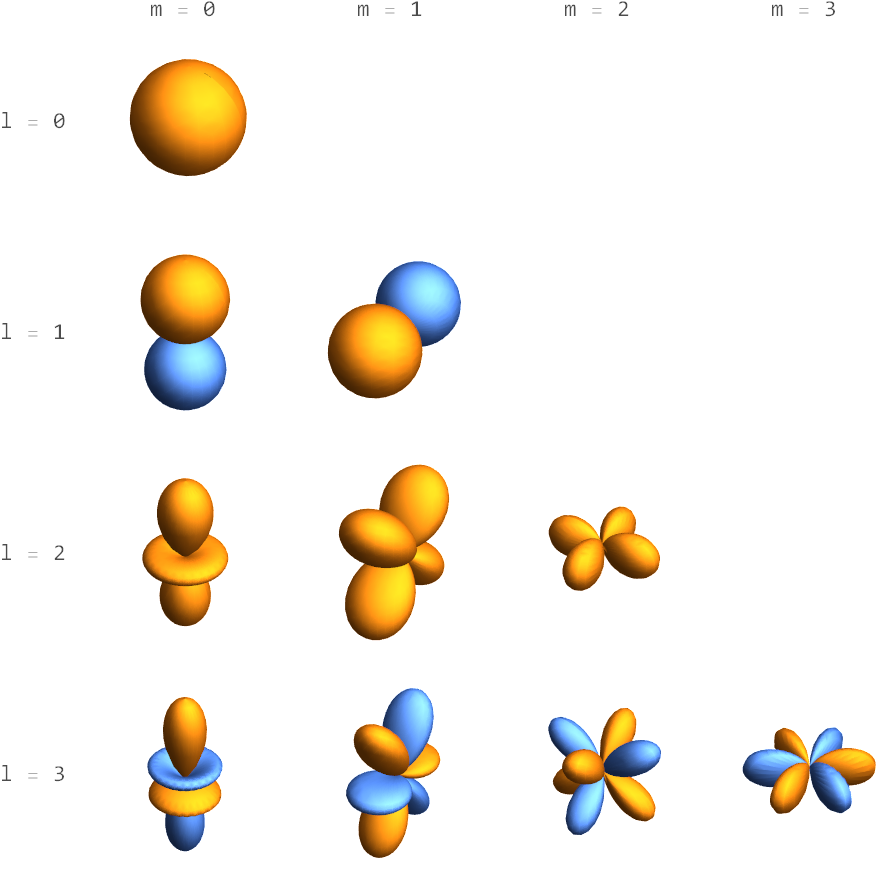
\includegraphics[width=0.5\textwidth]{angle_modes}
                \caption[]{Сферические угловые моды для нескольких $l$}
                \label{fig:angle_modes}
            \end{figure}

        %
        %
        %
        %%%%%%%%%%%%%%%%%%%%%%%%%%%%%%%%%%%%%%%%%%%%%%%%%%%%%%%%%%%%%%%%%%%
        %                        SUBSECTION                               %
        %%%%%%%%%%%%%%%%%%%%%%%%%%%%%%%%%%%%%%%%%%%%%%%%%%%%%%%%%%%%%%%%%%%
        %
        %
        %

        \subsection{Нахождение радиальных частей скалярных сферических мод}

            В данном пункте мы ограничимся скалярными модами $f_{l,m}(r,\theta,\varphi)$.

            Радиальные части сферических мод будем искать из \autoref{eq:wave_equation}. Будем отталкиваться от того, что оператор Лапласа $\Delta$ коммутирует с операторами $\Op{l}^2$ и $\Op{l}_{+} \Op{l}_{-}$, а значит имеет с ними общие собственные функции.

            Поскольку операторы повышения и понижения, $\Op{l}_{+}$ и $\Op{l}_{-}$, не содержат дифференцирования по $r$, искать радиальную часть имеет смысл только для базовой моды. Остальные моды будут иметь точно такую же радиальную часть и получаться из базовой моды путем применения операторов повышения и понижения.

            Решим задачу Штурма-Лиувилля для оператора Лапласа и базовой моды $f_{l}(r,\theta) = f(r) f_{l}(\theta)$:
            %
            \begin{equation}
                \Delta f(r) f_{l}(\theta) = - \lambda f(r) f_{l}(\theta) .
            \end{equation}
            %
            Это дифференциальное уравнение должно выполняться для любого $\theta$. Можно показать, что данное требование выполняется, если $f(r)$ удовлетворяет другому дифференциальному уравнению,
            %
            \begin{equation}
                r^2 f''(r) + 2 r f'(r) + (\lambda r^2 - l(l+1)) f(r) = 0 ,
            \end{equation}
            %
            решением которого являются сферические $J$- и $Y$-функции Бесселя, получаемые из обычных $J$- и $Y$-функций Бесселя по формулам:
            %
            \begin{equation}
                j_n(r) = \frac{\sqrt{\pi/2}}{\sqrt{r}} J_{n+\frac{1}{2}}(r) ; \quad
                y_n(r) = \frac{\sqrt{\pi/2}}{\sqrt{r}} Y_{n+\frac{1}{2}}(r) . \quad
            \end{equation}
            %
            Сферическая $Y$-функция Бесселя, однако, имеет расходимость при $r \to 0$, поэтому не определяет физически реализуемого решения.

            Итак, выбирая единственную константу равной единице, запишем (\autoref{fig:radial_modes})
            %
            \begin{equation}
                f(r) = j_l(\sqrt{\lambda} r) .
            \end{equation}
            %
            Полное решение тогда будет иметь вид:
            %
            \begin{equation}
                f_{l,m}(r,\theta,\varphi)
                    = j_l(\sqrt{\lambda} r) i^m \exp(- i m \varphi) P^m_l\qty(\cos\theta) .
            \end{equation}
            %
            \begin{figure}[h]
                \centering
                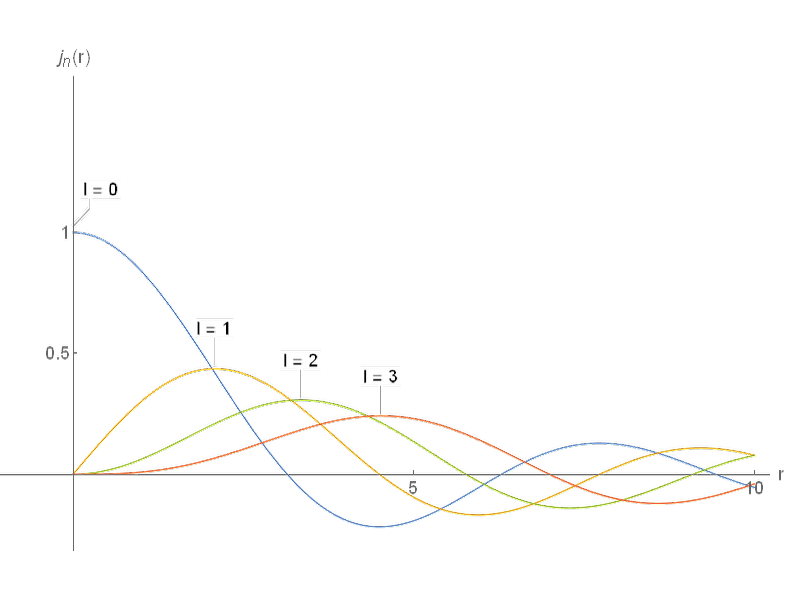
\includegraphics[width=0.5\textwidth]{radial_modes}
                \caption[]{Сферические радиальные моды для нескольких $l$}
                \label{fig:radial_modes}
            \end{figure}

        %
        %
        %
        %%%%%%%%%%%%%%%%%%%%%%%%%%%%%%%%%%%%%%%%%%%%%%%%%%%%%%%%%%%%%%%%%%%
        %                        SUBSECTION                               %
        %%%%%%%%%%%%%%%%%%%%%%%%%%%%%%%%%%%%%%%%%%%%%%%%%%%%%%%%%%%%%%%%%%%
        %
        %
        %

        \subsection{Векторные сферические моды}

            Применим теперь описанную и проверенную в скалярном случае методику к нахождению сферических мод векторного поля.

            Пусть векторное поле $\vb{a}$ задается своими контравариантными компонентами $a^k$ и удовлетворяет уравнению Лапласа:
            %
            \begin{equation}\label{eq:laplacian_sturm_liouville}
                \Delta \vb{a} = - \lambda \vb{a} .
            \end{equation}

            Для упрощения последующих выкладок и максимального \enquote{развязывания} компонент искомого поля решим следующую задачу. Как известно, базовая мода $\vb{a}_{l,0}$ не зависит от $\varphi$. Найдем разложение $\vb{a}_{l,0}$ на элементарные моды, т.е. моды, имеющие максимальное количество нулевых компонент. Поскольку оператор Лапласа линеен, это вполне допустимо.

            Рассмотрим поле $\vb{b}$ той же конфигурации, что и базовая мода, т.е. $b^k = b^k(r,\theta)$. Будем действовать оператором Лапласа на векторы, получаемые из $\vb{b}$ \enquote{вычеркиванием} отдельных компонент и постановкой на их место нулей, т.е. на $\qty{ b^1, 0, 0 }$, $\qty{ 0, b^2, 0 }$, \dots, $\qty{ 0, b^2, b^3 }$.

            Проделывая эту процедуру в сферических координатах $\qty(r, \theta, \varphi)$, мы обнаружим, что для многих конфигураций поля поставленная задача Штурма-Лиувилля для оператора Лапласа (\autoref{eq:laplacian_sturm_liouville}) в общем нетривиальном случае ($\lambda \neq 0$) неразрешима. Она разрешима лишь для трех конфигураций: $\vb{b}_{\mathrm{I}} = \qty{ b^r, b^\theta, 0 }$, $\vb{b}_{\mathrm{II}} = \qty{ 0, 0, b^\varphi }$ и, собственно, $\vb{b} = \qty{ b^r, b^\theta, b^\varphi } = \vb{b}_{\mathrm{I}} + \vb{b}_{\mathrm{II}}$. Назовем первые две из них $\mathrm{I}$ и $\mathrm{II}$ поляризациями.

            Таким образом, достаточно искать решение \autoref{eq:laplacian_sturm_liouville} для $\mathrm{I}$- и $\mathrm{II}$-поляризованного векторного поля. Поле общей конфигурации всегда может быть получено в виде их линейной комбинации.

            Применительно к электромагнитному полю конфигурации $\vb{E} = \qty{ E^r, E^\theta, 0 }$ и $\vb{E} = \qty{ 0, 0, E^\varphi }$ называются соответственно\footnotemark{} $TH$ и $TE$.

            \footnotetext{
                Некоторые авторы меняют эти определения местами.
            }

        %
        %
        %
        %%%%%%%%%%%%%%%%%%%%%%%%%%%%%%%%%%%%%%%%%%%%%%%%%%%%%%%%%%%%%%%%%%%
        %                        SUBSECTION                               %
        %%%%%%%%%%%%%%%%%%%%%%%%%%%%%%%%%%%%%%%%%%%%%%%%%%%%%%%%%%%%%%%%%%%
        %
        %
        %

        \subsection{Нахождение угловых частей векторных сферических мод}

            Найдем угловые части векторных сферических базовых мод. Для краткости обозначим угловую часть базовой $\mathrm{I}$-моды $\vb{a}(\theta)$, а $\mathrm{II}$-моды~--- $\vb{b}(\theta)$.

            Найдем вид $a^k$ и $b^k$, удовлетворяющий \autoref{eq:basemode_op_eq}. Для чего решим полученные из \autoref{eq:basemode_op_eq} дифференциальные уравнения:
            %
            \begin{equation}\begin{aligned}
                l (l + 1) a^1(\theta)
                    + \cot(\theta) \partial_\theta a^1(\theta)
                    + \partial^2_{\theta\theta} a^1(\theta) &= 0 \\
                (l^2 + l - \csc^2\theta) a^2(\theta)
                    + \cot(\theta) \partial_\theta a^2(\theta)
                    + \partial^2_{\theta\theta} a^2(\theta) &= 0 \\
                (l^2 + l - 2) b^3(\theta)
                    + 3 \cot(\theta) \partial_\theta b^3(\theta)
                    + \partial^2_{\theta\theta} b^3(\theta) &= 0
            \end{aligned}\end{equation}

            Решение последнего уравнения в приведенном виде представляет трудности. Оно, однако, допускает сведение к уравнению, по структуре идентичному второму. Представим $b^3(\theta)$ в виде двух множителей: $b^3(\theta) = f(\theta) s(\theta)$. После чего подействуем на $b^k$ оператором повышения и получим:
            %
            \begin{equation}
                \qty(\Op{l}_{+} b^k)^3 = - i \exp(i \varphi) \qty(
                    s(\theta) f'(\theta) + f(\theta) \qty(\cot(\theta) s(\theta) + s'(\theta))
                ) .
            \end{equation}
            %
            Сравнивая полученное выражение с
            %
            \begin{equation}
                \qty(\Op{l}_{+} a^k)^1 = - i \exp(i \varphi) \partial_\theta a^1(\theta) ,
            \end{equation}
            %
            выберем $s(\theta)$ так, чтобы
            %
            \begin{equation}
                \cot(\theta) s(\theta) + s'(\theta) = 0 .
            \end{equation}
            %
            Данное соотношение выполняется, если положить $s(\theta) = C \csc\theta$, где $C$~--- некоторая константа. Выберем ее равной $i$.

            Теперь, подставляя $b^k$ в \autoref{eq:basemode_op_eq}, получим дифференциальное уравнение на $f(\theta)$, идентичное уравнению на $a^2$:
            %
            \begin{equation}\label{eq:attached_legendre_pq}
                (l^2 + l - \csc^2\theta) f(\theta) + \cot(\theta) f'(\theta) + f''(\theta) = 0.
            \end{equation}

            Из математической физики известно, что уравнение вида \autoref{eq:attached_legendre_pq} является уравнением на присоединенные полиномы Лежандра первого порядка, $P_l^1(\cos\theta)$ и $Q_l^1(\cos\theta)$. Первое же уравнение уже известно и определяет полиномы Лежандра $P_l(\cos\theta)$ и $Q_l(\cos\theta)$. $Q$-полиномы, однако, не регулярны в нуле, потому не представляют собой физически реализуемого решения.

            Итак, запишем
            %
            \begin{equation}
                \vb{a} = \begin{pmatrix}
                    C_1 P_l(\cos\theta) \\
                    C_2 P_l^1(\cos\theta) \\
                    0
                \end{pmatrix} , \quad
                \vb{b} = \begin{pmatrix}
                    0 \\
                    0 \\
                    i C_3 \csc(\theta) P_l^1(\cos\theta)
                \end{pmatrix} .
            \end{equation}

            Получение общего вида производных мод представляет некоторые трудности. Компоненты поля не независимы. После применения оператора повышения (понижения) они \enquote{перемешиваются}, что мешает получению единообразной, пусть даже рекуррентной формулы. Производные моды предлагается искать применением соответствующих операторов. Стоит, однако, отметить, что $m$-я производная мода будет зависеть от $\varphi$ через множитель вида $(-i)^m \exp(i m \varphi)$.

            На \autoref{fig:angle_modes_vect_ii} изображена плотность энергии мнимой части поля $\vb{b}$. Видно, что она отличается от изображенной на \autoref{fig:angle_modes}. Кроме того, минимальным значением $l$ здесь является $l = 1$ в отличие от скалярного случая, где $l >= 0$.
            %
            \begin{figure}[h]
                \centering
                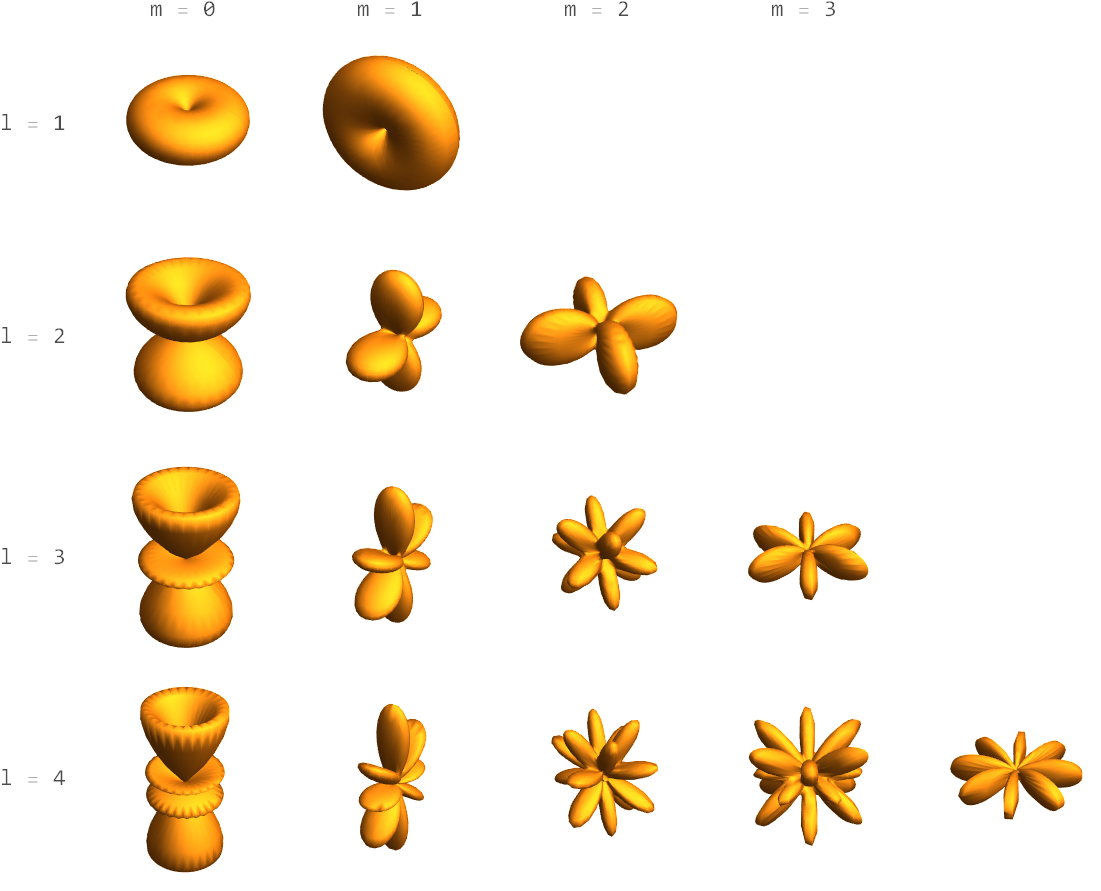
\includegraphics[width=0.5\textwidth]{angle_modes_vect_ii}
                \caption[]{Сферические угловые векторные моды для нескольких $l$}
                \label{fig:angle_modes_vect_ii}
            \end{figure}

    %
    %
    %
    %%%%%%%%%%%%%%%%%%%%%%%%%%%%%%%%%%%%%%%%%%%%%%%%%%%%%%%%%%%%%%%%%%%%%%%
    %                           SECTION                                   %
    %%%%%%%%%%%%%%%%%%%%%%%%%%%%%%%%%%%%%%%%%%%%%%%%%%%%%%%%%%%%%%%%%%%%%%%
    %
    %
    %

    \section{Выводы}

        В работе продемонстрировано применение методики Ли-генерации мод скалярного и векторного полей в трехмерном евклидовом пространстве. Многие математические выкладки были проделаны для риманова пространства общего вида, потому справедливы и в других классах риманова пространства, например на трехмерной сфере \cite{burlankov_tmf}.

        Применительно к векторным модам электромагнитного поля на данном этапе работы был получен вид только угловой части сферической базовой моды и приведена методика построения угловых частей производных мод. В дальнейшем будут получены также и радиальные части векторных мод.

        До сих пор наличие вмещающей сферы никак не учитывалось. Вопросом дальнейшего рассмотрения будет получение конкретного вида радиальных частей сферических мод в зависимости от размера сферы, иными словами граничных условий, накладываемых на рассматриваемое пространство.

        Заключительным этапом будет переход к термодинамике сферических резонаторов.

    %
    %
    %
    %%%%%%%%%%%%%%%%%%%%%%%%%%%%%%%%%%%%%%%%%%%%%%%%%%%%%%%%%%%%%%%%%%%%%%%
    %                        BIBLIOGRAPHY                                 %
    %%%%%%%%%%%%%%%%%%%%%%%%%%%%%%%%%%%%%%%%%%%%%%%%%%%%%%%%%%%%%%%%%%%%%%%
    %
    %
    %

    \bibliographystyle{../../../lib/doc/bib/utf8gost705s}
    \bibliography{%
        ../../../lib/doc/bib/resonators,%
        ../../../lib/doc/bib/physics,%
        ../../../lib/doc/bib/math%
    }

\end{document}
